\documentclass[times, 8pt,twocolumn]{article}
%\usepackage{ucs}
\usepackage{amsmath}
\usepackage{amsfonts}
\usepackage{amssymb}
%\usepackage{glossary}
%\usepackage{ucs}
\usepackage{listings}
%\usepackage{fontenc}
\usepackage{graphicx}
\usepackage{float}
\usepackage{color}
%\usepackage{tipa}
\usepackage{url}
\usepackage{hyperref}
%\usepackage{wrapfig}
%\usepackage{subfig}
\usepackage[left=1cm, top=1cm, right=1cm, bottom=1cm, nohead, nofoot]{geometry}
\title {RMI-based chat application: Papinho}
\author{Andon Tchechmedjiev, Jander Nascimento}
 \linespread{0.9}
 \usepackage[small,compact]{titlesec}
 \addtolength{\parskip}{-1.59mm}
\lstset{
basicstyle=\footnotesize,
tabsize=1,
breaklines=true,
language=java
}
 
\begin{document}
{\Large {\bf RMI-based chat application: Papinho}} \\
{\large {\bf {\it Andon Tchechmedjiev, Jander Nascimiento}}}
\section{Presentation}
\paragraph{} We have developed here a graphical RMI-based chat application named papinho as we were instructed.
The features implemented are the following : Sending of messages to a common public room, sending of private messages to any of the connected users on the public channel (except oneself), Changing one's name not only locally but on all the other clients as well, a full persistent history of the public channel on the server.
\paragraph{} The architecture we have chosen for our application is a classical server centric one. Namely, all the clients are synchronized to a central state kept on the server. All messages be they public or private messages, will always transit through the server, where logging will occur.
\section{Remote interfaces}
\paragraph{} We will first define the remote interfaces we used, as they constitute the basis of our application. There is one remote interface for the server application and one for the client application.
\subsection{Chat server side}
\paragraph{} Each of the methods of the remote interface listed in  table \ref{tab:serverprovide} represents the server part of one of the features above (except for the history).
\begin{small}
  \begin{table}[H]
  \begin{center}
      \begin{tabular}{ | l | p{5cm} |}
      \hline
      Method & Summary \\ \hline
      addClient & Add a client to the list of clients on the server side and notify the other clients; returns the list of users and the history to the client\\ \hline 
      removeClient & remove a client from the list of clients and notify the other clients\\ \hline
      sendMessage &  broadcast a message to all the clients (public chat), or to a specific client(private chat)\\ \hline
      clientNameChange & Change a user's name and notify the other clients \\ \hline
      \end{tabular}
  \end{center}
  \caption{Server Side remote interface methods}
  \label{tab:serverprovide}
  \end{table}
\end{small}
\subsection{Chat client side}
\paragraph{}Table \ref{tab:clientprovide} lists the remote methods for the server as well as a short description:
\begin{small}
  \begin{table}[H]
  \begin{center}
      \begin{tabular}{ | l | p{5cm} |}
      \hline
      Method & Summary \\ \hline
      addClient & Add a client to the list of clients on the client side \\ \hline 
      removeClient & remove a client from the list of clients on the client side \\ \hline
      receiveMessage & Add a new message to the main view \\ \hline
      receivePrivateMessage &  Add a new message to the appropriate private chat window \\ \hline
      changeClientName & Change the username in the list of clients on the client side \\ \hline
      \end{tabular}
  \end{center}
  \caption{Client Side remote interface methods}
  \label{tab:clientprovide}
  \end{table}
  \end{small}
\section{History and persistence}
\paragraph{} Here, we handle the persistence of the history, by serializing the {\it History} class directly to the disk, namely {\it bean serialization}. We also use the Proxy design pattern for the instantiation of the right DataSource. 
\section{Graphical User Interface}
\paragraph{} The Graphical User Interface(GUI) allows the user to interact with the application in a more intuitive and convivial way. Our graphical interface was implemented using the swing library as well a the Netbeans interface editor.
\paragraph{} Figure \ref{fig:papinho1} illustrates the main frame of our application, which contains: on the bottom left the text input field, in the bottom right, the Send button, on the top right side the user list and on the top left side the output text field (which supports colours for the usernames). The menu bar allow access to some useful function. 
\paragraph{} In the File menu can be found an {\it Options} menu item, which displays the dialogue that allows changing name, as well as the {\it Connect} menu item opening the dialogue which allows to connect to the server. Once the client is connected, the {\it Disconnect} menu item replaces {\it Connect}. 
\paragraph{} While there is no text in the input field, the send button is disabled, and the action of the Send button is supplemented by a press on the key Enter. As for the help menu it just contains a menu item that displays the about dialogue. 
\paragraph{} When a private chat is initiated, a private chat window pops up, in which it is possible to talk privately to whoever is on the other side of the line.
\begin{figure} [H]
    \centering
    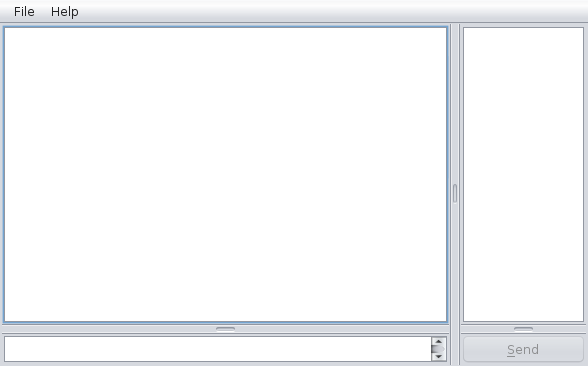
\includegraphics[scale=0.28]{img/mainscreen.png}
    \caption{Main Window} 
    \label{fig:papinho1}
\end{figure}
\section{Networking and security issues}
\paragraph{} Due to Java's default security policy, it is necessary to write a security policy file so as to allow clients to connect to our server remotely ( by default only connections incoming from localhost are authorized). Additionally, we needed to authorize the use of shutdown hooks as we use them to perform cleanup operations when the server JVM exits. Our policy file is exhibited in listing \ref{policyfile}. The policy file tu use is specified at runtime with -Djava.security.policy=./server.policy

\begin{lstlisting}[caption={Policy file},label=policyfile]
grant {
  permission java.security.AllPermission;
  permission java.net.SocketPermission "*:*", "accept,listen,connect,resolve";
  permission java.lang.RuntimePermission "shutdownHooks";
};
\end{lstlisting}

\paragraph{} We had a problem connecting clients from actual different hosts to the server, and as it turns out, the problem was that the server was bound to the wrong network interface. Indeed the UnicastRef returned to the clients pointed the ip address of this wrong interface, which in turn prevented the clients from connecting. In order to solve the problem, we had to manually specify the hostname to which to bind the server (bind in Socket terms not in RMI terms) with the runtime option -Djava.rmi.server.hostname=ipoftherightinterface.


\end{document}
